%!TEX root = ../thesis.tex
% Pipeline of the DemoDraw system: technical details

\section{Generation Pipeline}

\systemname{} has four main components (Figure~\ref{fig:pipeline}):
%
a \emph{motion capture} engine to record joint data from the author's demonstration and apply it to a 3D avatar;
%
a \emph{speech recognition} engine to process speech input for commands and motion labels;
%
a \emph{motion analysis} algorithm to partition recorded motion and identify salient joint movements for each illustration segment;
%
and an \emph{illustration rendering} engine to visualize the avatar and motion segments with different effects.
% , and a module to handle user interaction.
%
% Our novel techniques enables motion segmentation by combining speech and motion inputs. Our interaction model allows users to modify the rendered illustrations interactively by demonstrations.
These components combine into an interactive and iterative system pipeline to translate demonstrations into motion diagrams.
A notable technical contribution is our motion segmentation algorithm combining speech labels and joint motion streams.
%
\systemname{} is implemented using C\# in Unity 5. %\footnote{\url{https://unity3d.com}}.
It runs interactively on a Macbook Pro with Windows Bootcamp (2.5 GHz Intel Core i7 processor and 16 GB memory).
%
Below we describe the design and implementation of each component.

\begin{figure}[t]
  \centering
  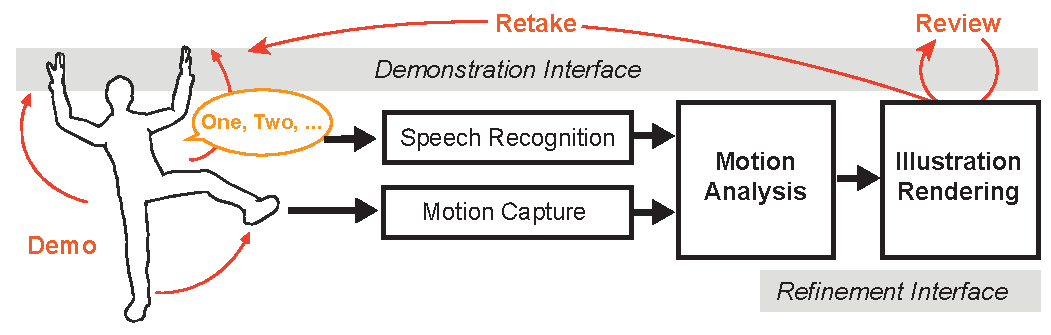
\includegraphics[width=0.8\columnwidth]{\demodraw/fig/pipeline/pipeline}
  \caption{\systemname{} system components and pipeline.}
  \label{fig:pipeline}
\end{figure}

% ---------------------------------------------------------------

\subsection{Motion Capture}

In support of our design goal to enable low-effort iteration within tasks, the motion capture component provides real-time feedback during demonstrations so authors can monitor their performance accordingly.
We capture position and joint angles of a simplified 25-joint skeleton using a Kinect2 sensor and the Kinect SDK 2.0. %\footnote{\url{https://dev.windows.com/en-us/kinect}}.
%\subsubTitleBold{Motion Re-targeting}
The real-time joint data is applied to a generic 3D human model (an ``avatar'') using forward kinematics enabled by a modified Unity asset\footnote{\url{https://www.assetstore.unity3d.com/en/\#!/content/18708}}.

% ---------------------------------------------------------------

\subsection{Speech Recognition}
Speech is used when recording a demonstration to label motions (e.g., ``one, two, ...'') and for recording and navigation commands (e.g. ``Start, Stop, Retake'' or ``Replay, Next, Play'') -- see Figure~\ref{fig:DemoDrawUI} for the speech commands that \systemname{} supports.
\dan{I made these consistent with new Figure 4}
%
We recognize both types of speech using the Microsoft speech recognition library\footnote{\url{https://msdn.microsoft.com/en-us/library/hh361572}} to process audio captured by the Kinect microphone array.
During recording, the start time, duration, and confidence of each motion label are logged for use in the motion analysis algorithm.

% ---------------------------------------------------------------

\begin{figure}[!t]
  \centering
  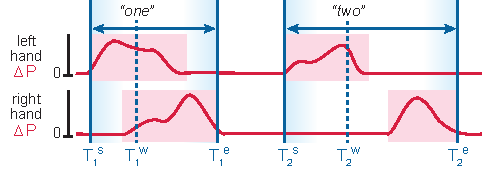
\includegraphics[width=0.8\columnwidth]{\demodraw/fig/motion_analysis/analysis2}
  \caption{Illustration of motion analysis algorithm (two joints shown due to space): significant moving periods of joint movements (pink) are mapped to speech labels to define motion segments (blue). Note the right hand period is mapped to \iquote{two} because it begins shortly after the left hand period.}
   \label{fig:segmentation}
\end{figure}

\subsection {Motion Analysis}

Our motion analysis algorithm translates a multi-part demonstration recording into a sequence of labeled time segments, each with one or more salient joint motions and a keyframe of joint positions for a representative body pose (see Figure~\ref{fig:segmentation} for an illustration of the approach).
Formally, given a set of $n$ speech labels $\{w_1, w_2, ..., w_n\}$ that end at latency-corrected times $\{T_1^w, T_2^w, ..., T_n^w\}$, our algorithm associates each speech label $w_i$ with a \emph{motion segment}, of which the start and end time are denoted as [$T_i^s$, $T_i^e$] where $T_i^s \leq T_i^w \leq T_i^e$. Each motion segment includes a set of $k$ salient joints $\{j_i^1, ..., j_i^k\}$ and keyframe time $T_i^{key}$ between [$T_i^s$, $T_i^e$].
It is then sent to the Illustration Rendering engine to create a motion illustration in a multi-part sequence.

Human motion segmentation and activity understanding has been well studied in computer vision and graphics \cite{Aggarwal:2011:HAA:1922649.1922653}. We adopted a spacetime approach to identify salient motion sequences in 3D space.
%
However, in our scenario such as dancing, movements may not necessarily encode a semantic meaning for automatic recognition, such as ``walking'' or ``throwing (a ball)'' in previous research. Therefore, our approach combines the user's speech labels, similar to a scene segmentation method used in DemoCut~\cite{Chi:2013:DGC:2501988.2502052}.
%
We make two assumptions about the synchronized data streams of speech labels and joint movements:
1) authors make short pauses between motions to be grouped, i.e., $T_i^e < T_{i+1}^s$, and
2) the speech label utterances overlap or closely occur with at least one joint motion.
%
These assumptions are practical since authors often pause for a moment to prepare for demonstrating the next movement in a step-by-step sequence.

% EUCLIDEAN DISTANCE
\subsubTitleBold{Motion Segmentation}
To determine a motion segment of [$T_i^s$, $T_i^e$] for each speech label $w_i$ that ends at $T_i^w$, we begin by identifying all \emph{moving periods} of significant joint movements (pink rectangles in Figure~\ref{fig:segmentation}) for 8 joints $J$: the 5 end-effectors (head, hands, feet), 2 knees, and the body root.
%
To filter jittery movements, joints are considered moving if smoothed inter-frame differences in absolute Euclidean distance are greater than a threshold.
%
Specifically, for each joint $j \in J$ of a frame $r$ at time $t$, the average difference in position between two adjacent frames $\Delta P = |P^r-P^{r-1}|$ is computed over the subsequent half second (15 frames).
%
If this moving average is greater than 0.05$m/s$, then joint $j$ of a frame is labeled as ``moving'', marked as $m_j^r$.
This is repeated on all frames and all joints.
Next, of the entire motion recording for joint $j$, we combine all the consecutive $\{m_j^r, m_j^{r+1}, ...\}$ into a joint moving period $M_j$.

Once a list of moving periods $\{M_j^1, M_j^2, ...\}$ for joint $j$ is determined, we begin labeling each $M_j^m$ at [$T_{m}^s$, $T_{m}^e$] to map to a speech label $w_i$ at time $T_i^w$ where $T_m^s \leq T_i^w \leq T_m^e$. In other words, the speech utterance occurs during or near to a joint movement (illustrated as dashed lines crossing pink rectangles in Figure~\ref{fig:segmentation}).
%
After all moving periods are mapped to speech labels for all major joints in $J$, the start and end time [$T_i^s$, $T_i^e$] of the motion segment for label $w_i$ are set to the minimum start time and maximum end time across all mapped joint movement periods.

\subsubTitleBold{Joint Salience Identification}
The salient joints $\{j_i^1, ..., j_i^k\}$ are defined by the set of all joints that were mapped based on significant moving periods.

% KEY FRAME
\subsubTitleBold{Key Pose Selection}
A key pose is used to represent a motion segment in an illustration. Based on our informal experiment, it is often the end state of movements as motion arrows are pointed toward this end goal (see the Figure~\ref{fig:pipeline} for example). Therefore, we set a key pose at the end of a motion segment, i.e., $T_i^{key} = T_i^e$.

\subsubTitleBold{Motion Retake}
When retaking a partial demonstration with one or more speech labels $\{w_i', w_{i+1}', ...\}$, the full motion analysis algorithm is run on the new recording. New motion segments then replace the original segments by mapping $w_i'$ with $w_i$.

% ---------------------------------------------------------------

\subsection{Illustration Rendering}

The Illustration Rendering engine generates a motion illustration for each motion segment of speech label $w_i$ (bounded by [$T_i^s$, $T_i^e$]). There are two related rendering tasks: the body pose and the motion depiction style.

\subsubTitleBold{Body Pose}
The body pose is determined by all joint positions at keyframe time $T_i^{key}$.
We use standard Non-Photorealistic Rendering (NPR)~\cite{gooch1998non} techniques to render the 3D human model in a stylized manner that abstracts away distracting details. Specifically, we support contour-only, filled silhouette, and flat-shaded rendering styles
(see Figure~\ref{fig:DemoDrawRefinementUI}a left for examples).

\subsubTitleBold{Line and Arrow Depiction Style}
Based on Cutting's criteria~\cite{cutting_representing_2002} and our survey of motion illustrations, we use lines with arrowheads as the default depiction style for visualizing joint movements.
This style is rendered as follows:
%
For each salient joint of a motion segment, the absolute joint positions in world space over the period [$T_i^s$, $T_i^e - \epsilon$] are used to construct a 3D poly-line using Catmull-Rom interpolation. Rather than visualizing the entire path, we set $\epsilon$ to be 0.5 seconds to visually point the arrow toward the key pose at $T_i^e$.
Two 3D cones are positioned collinear with the last two polyline positions to form arrowheads for both the beginning and the end of a line.
%
Although the poly-line is 3D, it is shaded to appear 2D.
%
All arrows are colored red by default to contrast with the avatar, a common technique for layering information~\cite{tufte1990envisioning}.

For some motions, visualizing absolute joint positions might not be suitable.
For example, for a two-foot jump with a two-hand waving motion (see Figure~\ref{fig:DemoDrawRefinementUI}c), our algorithm will mark all major joints as salient and generate multiple arrows showing the jump movement, but fail to convey the hand waving.
%
Authors can choose to visualize joint motions \textit{relative} to the spine instead,
triggering the same motion analysis algorithm described above to be re-run using relative motion.
In this way, the same movements would be shown more concisely with a single up arrow (for the overall jump direction) and two curve arrows (for the hand movements).

\subsubTitleBold{Other Adjustments}
Authors can review the results using the \phaseI{} or \phaseII{}. With the latter, line weight, arrowhead sizes, and color can be adjusted and re-rendered in real-time using graphical widgets (see Figure~\ref{fig:DemoDrawRefinementUI}a). Arrows can also be re-positioned to increase the offset ($\delta$) by direct manipulation dragging.
%
Considering some movements cannot be easily seen from the default front camera viewpoint (such as those parallel to the XZ plane, see Figure~\ref{fig:demodraw_teaser}c top-right), our UI enables the selection of four other camera angles ($\theta$), including three-quarter front views (45$^{\circ}$ and -45$^{\circ}$) and profile views (90$^{\circ}$ and -90$^{\circ}$), all at the eye level. These discrete choices simplify control, but of course it would be possible to select any viewing angle given the 3D avatar and joint information. By default, 8 main joints are analyzed and illustrated, but any of the 25 body joints can be explicitly selected for illustration using the interface.

\subsubTitleBold{Stroboscopic Depiction Style}
Cutting~\cite{cutting_representing_2002} noted stroboscopic effects are also effective, and we found examples of illustrations with a sequence of overlaid semi-transparent body poses in our survey.
%
Therefore, authors can select a stroboscopic depiction style in the \phaseII{} (see Figure~\ref{fig:DemoDrawRefinementUI}b).
The style is rendered by compositing multiple semi-transparent renderings of intermediate body poses between $T_i^s$ to $T_i^e$ behind a rendering of the representative pose at keyframe time $T_i^{key}$.
Authors can adjust the number of intermediate poses $n$ (the default is 3 poses) and the horizontal overlap ratio $\rho$ between intermediate pose renderings can be adjusted to stack them up ($\rho=100\%$) or spread them out ($\rho=0$ is the default).

% Authors can then selectively combine these frames by specifying visual parameters, including numbers of frames to show, distance between frames, and whether to apply motion arrows. Our system will automatically adjust the distance and transparency values of selected frames and compose into a diagram.

\subsection{Results}
The \systemname{} pipeline is capable of generating expressive and clear motion illustrations. In Figure~\ref{fig:demodraw_teaser}c, motion arrows show the upper body motion (top left), hand waving back and forth (top middle), and hand circular motion (bottom right). Whole body motions can also be visualized (bottom left), and can be especially helpful when motions are best viewed from a different angle, such as the side view (top right).
%
In Figure~\ref{fig:demodraw_teaser}d, stroboscopic effect depicts the transition from the start pose to the end pose, which can be rendered as a sequence (top left) or in one combined pose (bottom left). A combination of this effect with motion arrows creates a compact, integrated illustration (top and bottom right).

\dan{Disclose what happens if assumptions don't hold or other problems with the pipeline. (this paragraph may migrate elsewhere).}
